\section{第十周数值分析中期练习}
\subsection{三次插值}
\begin{ex}
已知 $y=f(x)$ 的在部分节点上的函数值如下表所示:
\begin{table}[H]
	\centering
	\begin{tabular}{|c|c|c|c|c|}
		\hline$x_i$ & -2 & 0 & 1 & 2 \\
		\hline$f\left(x_i\right)$ & -7 & 1 & 2 & 9 \\
		\hline
	\end{tabular}
\end{table}
	试构造三次插值多项式, 并估计在 $x=1.3$ 处的值。
\end{ex}
\lstinputlisting[language=matlab]{w10/q1.m}
\qa $x^3+1$;
3.1970e+000
\subsection{最小二乘法}
\begin{ex}
	已知实验数据如下:
	\begin{table}[H]
		\centering
		\begin{tabular}{|c|c|c|c|c|c|c|}
			\hline$x_i$ & 10 & 11 & 12 & 13 & 14 & 15 \\
			\hline$f\left(x_i\right)$ & 20 & 23 & 25 & 27 & 26 & 28 \\
			\hline
		\end{tabular}
	\end{table}
	请列出用最小二乘法求线性及二次拟合函数的方程组。
\end{ex}
\lstinputlisting[language=matlab]{w10/q2.m}
\qa 
\begin{flalign*}
	\begin{split}
		y=\frac{51\,x}{35}+\frac{1863096274418193}{281474976710656}.
	\end{split}&
\end{flalign*}
\begin{flalign*}
	\begin{split}
		y=-\frac{683582086296581\,x^2}{2251799813685248}+\frac{5092686542910377\,x}{562949953421312}-\frac{5619446856466419}{140737488355328}.
	\end{split}&
\end{flalign*}
\begin{figure}[H]
	\centering
	\subfloat[一次拟合多项式]{\includegraphics[width = 0.5\linewidth]{w10/q21.eps}}
	\hfill
	\subfloat[二次拟合多项式]{\includegraphics[width = 0.5\linewidth]{w10/q22.eps}}
	\caption{最小二乘法}
\end{figure}
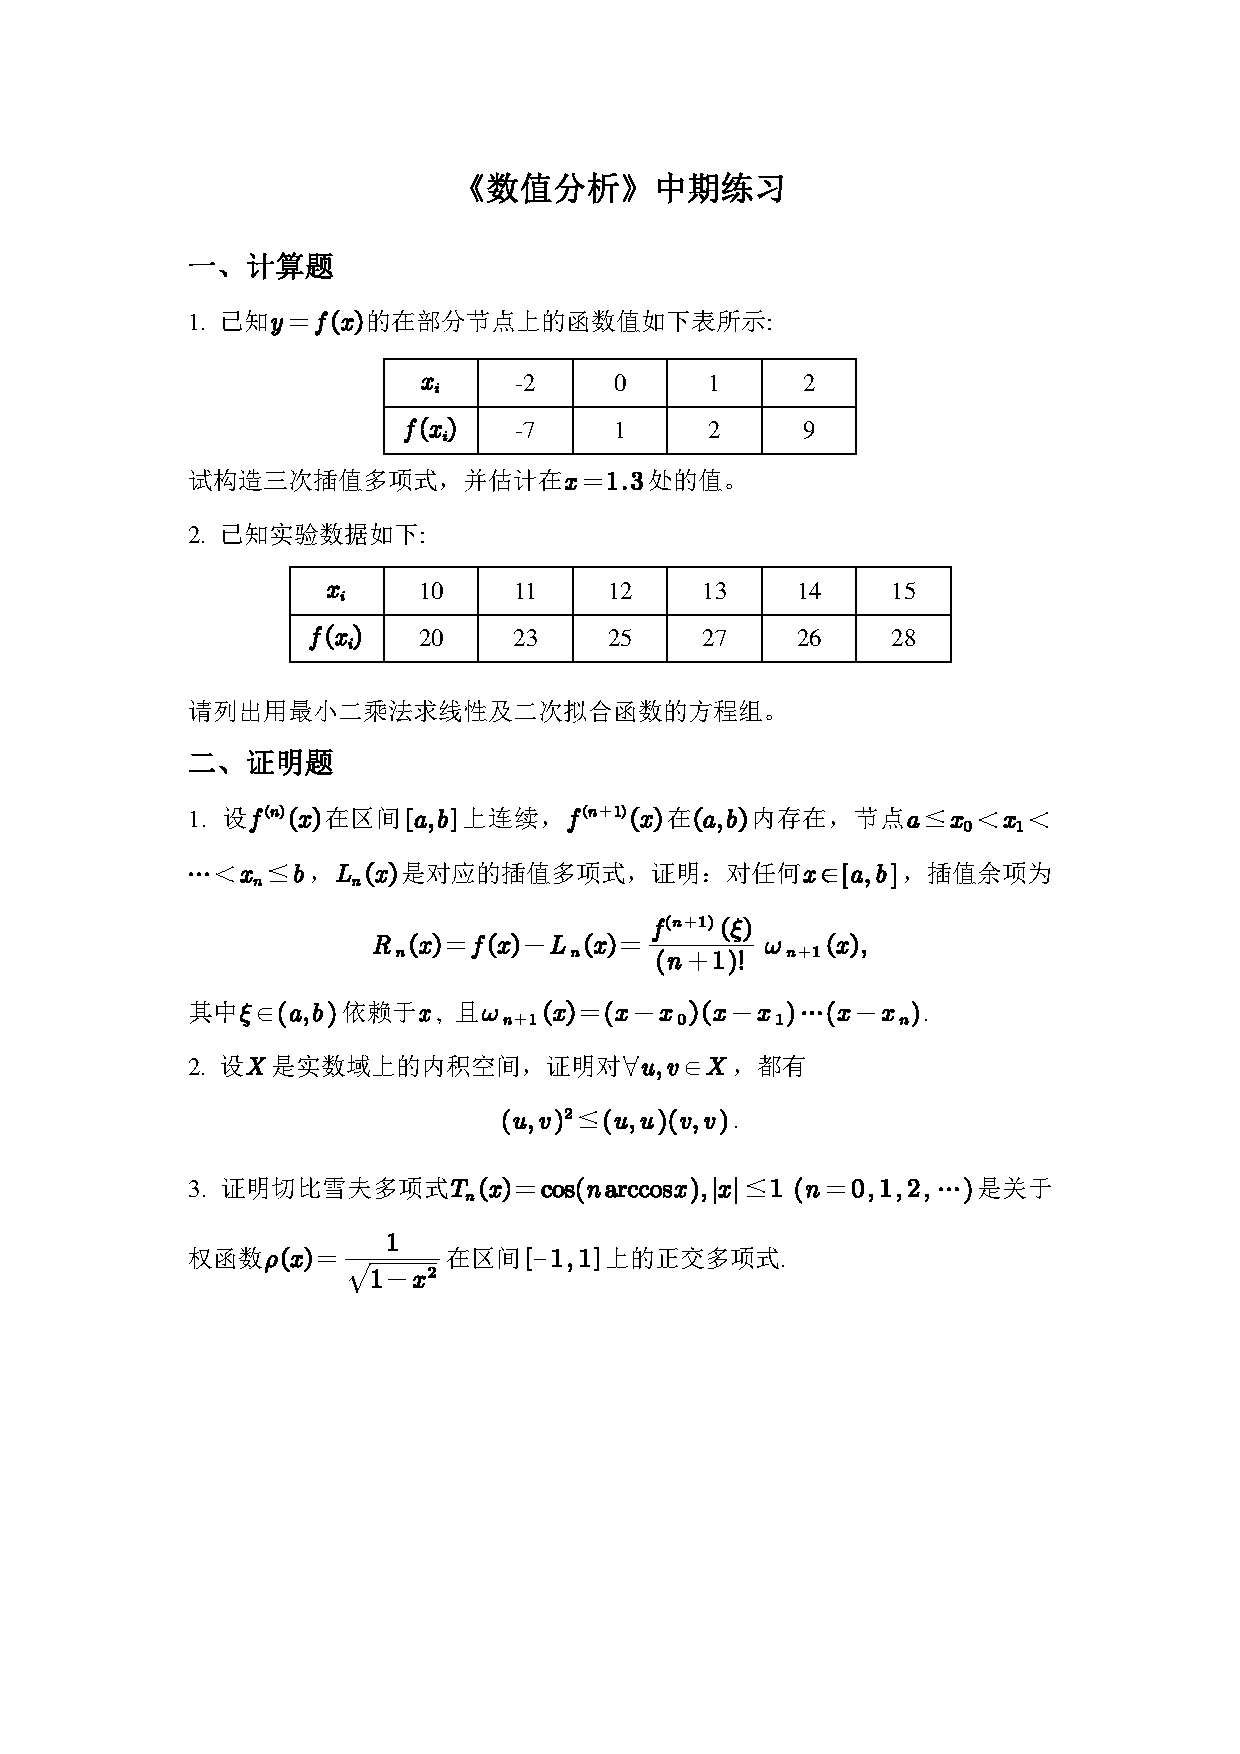
\includepdf{w10/fig.pdf}

